\documentclass{article}
\usepackage{longtable}
\usepackage[utf8]{inputenc}
\usepackage{graphicx}
\usepackage{amsmath}
\usepackage{amssymb}
\usepackage{tcolorbox}
\tcbuselibrary{breakable}
\usepackage{listings}
\usepackage{xcolor}
\usepackage{geometry}
\usepackage{titlesec}
\usepackage{float} % For [H] float placement

\geometry{a4paper, margin=1in}

% Define colors for tcolorbox
\definecolor{titlebg}{RGB}{0,70,110}
\definecolor{boxbg}{RGB}{240,248,255}

% Listing style for Arduino code
\lstdefinestyle{arduino}{
    language=C++,
    basicstyle=\small\ttfamily,
    keywordstyle=\color{blue},
    commentstyle=\color{green!60!black},
    stringstyle=\color{red},
    numbers=left,
    numberstyle=\tiny\color{gray},
    stepnumber=1,
    numbersep=5pt,
    backgroundcolor=\color{boxbg},
    frame=single,
    framerule=0pt,
    rulecolor=\color{white},
    breaklines=true,
    postbreak=\mbox{\textcolor{red}{$\hookrightarrow$}\space},
    tabsize=2,
    showstringspaces=false
}

% Custom title page
\title{
    \vspace{2cm}
    \textbf{MOD-7 Asynchronous Counter using T Flip-Flops} \\
    \large Design, Implementation and Testing Report
    \vspace{1cm}
}
\author{
   Krishna Patil - EE24BTECH11036 \\
   Deepak Ahirwar - EE24BTECH11014
}
\date{\today}

\begin{document}

\maketitle
\thispagestyle{empty}

\clearpage

\section*{Abstract}
\begin{tcolorbox}[colback=boxbg,colframe=titlebg,title=Abstract,breakable]
The MOD-7 asynchronous counter successfully counts from 0 to 6 before automatically resetting to 0. This report details the design, implementation, and testing of the counter using JK flip-flops configured as T flip-flops, with an Arduino providing the clock signal. The counter displays its state on a 7-segment display and its operation is verified through oscilloscope measurements.
\end{tcolorbox}

\tableofcontents

\section{Theoretical Background}
\subsection{T Flip-Flop Fundamentals}
\begin{tcolorbox}[colback=boxbg,colframe=titlebg,title=T Flip-Flop Fundamentals,breakable]
The T flip-flop (Toggle flip-flop) gets its name from its ability to toggle its output state. It has a single input T that controls its behavior:

\begin{itemize}
    \item When T=1, the output toggles (changes state) on each clock pulse
    \item When T=0, the output maintains its current state with no change
\end{itemize}

The characteristic equation that defines a T flip-flop's behavior is:

\begin{equation}
    Q_{n+1} = T'Q_n + TQ_n'
\end{equation}

Where $Q_n$ is the present state, $Q_{n+1}$ is the next state, and T is the toggle input.
\end{tcolorbox}

\subsection{Converting JK Flip-Flop to T Flip-Flop}
\begin{tcolorbox}[colback=boxbg,colframe=titlebg,title=JK to T Flip-Flop Conversion,breakable]
Since dedicated T flip-flop ICs are not commonly available, JK flip-flops are used to implement them. The conversion is straightforward:

\begin{itemize}
    \item Connect both J and K inputs to the same signal source (T input)
    \item When J=K=0, the flip-flop holds its current state
    \item When J=K=1, the flip-flop toggles on each clock pulse
\end{itemize}

This connection arrangement makes the JK flip-flop behave exactly like a T flip-flop.
\end{tcolorbox}

\section{Circuit Design}
\subsection{Circuit Connections}
\begin{tcolorbox}[colback=boxbg,colframe=titlebg,title=Circuit Connections,breakable]
The complete circuit connections for the MOD-7 asynchronous counter are shown in Table~\ref{tab:circuit}.
\end{tcolorbox}

\begin{center}
\small % Makes the table slightly more compact
\begin{longtable}{|>{\raggedright}p{3cm}|>{\raggedright}p{2cm}|>{\raggedright}p{6cm}|}
    \caption{Connections for Mod-7 Asynchronous Counter with Display}
    \label{tab:circuit}\\
    \hline
    \textbf{Component} & \textbf{Pin} & \textbf{Connection} \\
    \hline
    \endfirsthead
    
    \hline
    \multicolumn{3}{|c|}{\textbf{Continued from previous page}} \\
    \hline
    \textbf{Component} & \textbf{Pin} & \textbf{Connection} \\
    \hline
    \endhead
    
    \hline
    \multicolumn{3}{|r|}{\textbf{Continued on next page}} \\
    \endfoot
    
    \hline
    \endlastfoot
    
    \multicolumn{3}{|l|}{\textbf{Arduino Connections}} \\
    \hline
    Arduino & Pin 13 & Clock Input to First 7476 Flip-Flop \\
    \hline
    
    \multicolumn{3}{|l|}{\textbf{7476 (First Flip-Flop - Q1)}} \\
    \hline
    7476 (IC1) & VCC (Pin 16) & +5V \\
    7476 (IC1) & GND (Pin 8) & 0V (Ground) \\
    7476 (IC1) & J1, K1 & +5V (HIGH) \\
    7476 (IC1) & CLK1 & Arduino Pin 13 (Clock) \\
    7476 (IC1) & Q1 (Pin 15) & Clock for Second Flip-Flop \\
    7476 (IC1) & PRE1, CLR1 & +5V (HIGH) \\
    7476 (IC1) & CLR1 & Input from 7410 NAND Gate \\
    \hline
    
    \multicolumn{3}{|l|}{\textbf{7476 (Second Flip-Flop - Q2)}} \\
    \hline
    7476 (IC2) & VCC (Pin 16) & +5V \\
    7476 (IC2) & GND (Pin 8) & 0V (Ground) \\
    7476 (IC2) & J2, K2 & +5V (HIGH) \\
    7476 (IC2) & CLK2 & Q0 Output from First Flip-Flop \\
    7476 (IC2) & Q2 (Pin 15) & Input to 7410 NAND Gate \\
    7476 (IC2) & PRE2 & +5V (HIGH) \\
    7476 (IC2) & CLR2 & Input from 7410 NAND Gate \\
    \hline
    
    \multicolumn{3}{|l|}{\textbf{7476 (Third Flip-Flop - Q3)}} \\
    \hline
    7476 (IC3) & VCC (Pin 16) & +5V \\
    7476 (IC3) & GND (Pin 8) & 0V (Ground) \\
    7476 (IC3) & J3, K3 & +5V (HIGH) \\
    7476 (IC3) & CLK3 & Q1 Output from Second Flip-Flop \\
    7476 (IC3) & Q3 (Pin 15) & Input to 7410 NAND Gate \\
    7476 (IC3) & PRE3 & +5V (HIGH) \\
    7476 (IC3) & CLR3 & Input from 7410 NAND Gate \\
    \hline
    
    \multicolumn{3}{|l|}{\textbf{7410 (NAND Gate for Reset)}} \\
    \hline
    7410 (IC4) & VCC (Pin 14) & +5V \\
    7410 (IC4) & GND (Pin 7) & 0V (Ground) \\
    7410 (IC4) & Input 1 & Q0 from First 7476 \\
    7410 (IC4) & Input 2 & Q1 from Second 7476 \\
    7410 (IC4) & Input 3 & Q2 from Third 7476 \\
    7410 (IC4) & Output & CLR of All 7476 Flip-Flops \\
    \hline
    
    \multicolumn{3}{|l|}{\textbf{7447 (BCD to 7-Segment Decoder)}} \\
    \hline
    7447 (IC5) & VCC (Pin 16) & +5V \\
    7447 (IC5) & GND (Pin 8) & 0V (Ground) \\
    7447 (IC5) & A (Pin 7) & Q0 from First Flip-Flop \\
    7447 (IC5) & B (Pin 1) & Q1 from Second Flip-Flop \\
    7447 (IC5) & C (Pin 2) & Q2 from Third Flip-Flop \\
    7447 (IC5) & D (Pin 6) & GND (Always 0 for MOD-7 Counter) \\
    7447 (IC5) & Outputs (a-g) & Corresponding Pins of 7-Segment Display \\
    \hline
    
    \multicolumn{3}{|l|}{\textbf{7-Segment Display}} \\
    \hline
    7-Segment & a & Output a from 7447 \\
    7-Segment & b & Output b from 7447 \\
    7-Segment & c & Output c from 7447 \\
    7-Segment & d & Output d from 7447 \\
    7-Segment & e & Output e from 7447 \\
    7-Segment & f & Output f from 7447 \\
    7-Segment & g & Output g from 7447 \\
    7-Segment & Common Anode & +5V via 220$\Omega$ Resistor \\
    \hline
\end{longtable}
\end{center}

\begin{figure}[H]
    \centering
    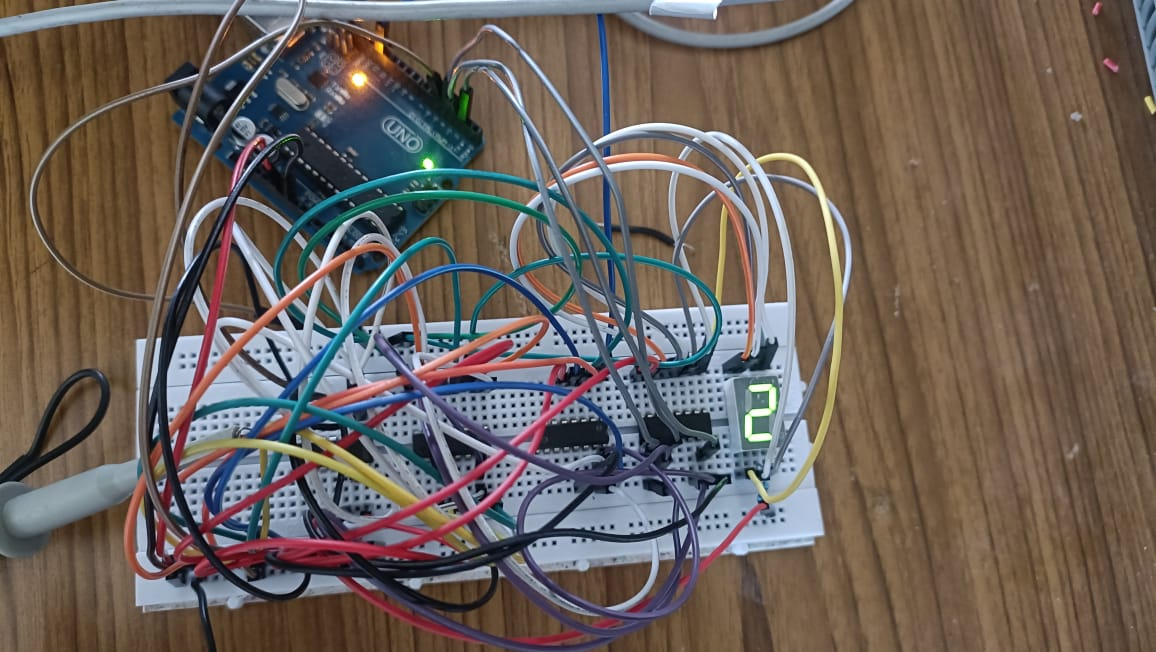
\includegraphics[width=0.7\textwidth]{figs/Circuit.jpeg} % Add your image file
    \caption{Circuit Diagram of Mod-7 Counter}
\end{figure}

\subsection{T Flip-Flop Implementation}
\begin{tcolorbox}[colback=boxbg,colframe=titlebg,title=T Flip-Flop Implementation,breakable]
Each JK flip-flop is configured as a T flip-flop by:

\begin{itemize}
    \item Connecting both J and K inputs to logical HIGH (VCC)
    \item This makes them function in "toggle mode" on each clock pulse
    \item The clock input of the first flip-flop comes from the Arduino
    \item The clock inputs of subsequent flip-flops come from the previous flip-flop's output
\end{itemize}
\end{tcolorbox}

\subsection{Counter Architecture}
\begin{tcolorbox}[colback=boxbg,colframe=titlebg,title=Counter Architecture,breakable]
The asynchronous MOD-7 counter consists of:

\begin{itemize}
    \item Three JK flip-flops (configured as T flip-flops) forming a binary counter chain
    \item A reset detection circuit using a 3-input NAND gate
    \item A display decoder and 7-segment display
\end{itemize}

The counter operates as follows:

\begin{itemize}
    \item The first flip-flop (Q0) receives the clock from Arduino and toggles on each clock pulse
    \item Q0 output clocks the second flip-flop (Q1), which toggles when Q0 transitions from HIGH to LOW
    \item Q1 output clocks the third flip-flop (Q2), which toggles when Q1 transitions from HIGH to LOW
    \item The NAND gate monitors all three outputs and resets the counter when it would reach state "111"
\end{itemize}
\end{tcolorbox}

\section{Truth Tables and State Diagrams}
\subsection{JK Flip-Flop Truth Table}
\begin{tcolorbox}[colback=boxbg,colframe=titlebg,title=JK Flip-Flop Truth Table,breakable]
\centering
\begin{tabular}{|c|c|c|c|l|}
\hline
J & K & Q(n) & Q(n+1) & Operation \\ \hline
0 & 0 & 0 & 0 & No change \\ \hline
0 & 0 & 1 & 1 & No change \\ \hline
0 & 1 & 0 & 0 & Reset \\ \hline
0 & 1 & 1 & 0 & Reset \\ \hline
1 & 0 & 0 & 1 & Set \\ \hline
1 & 0 & 1 & 1 & Set \\ \hline
1 & 1 & 0 & 1 & Toggle \\ \hline
1 & 1 & 1 & 0 & Toggle \\ \hline
\end{tabular}
\end{tcolorbox}

\subsection{MOD-7 Counter State Transition Table}
\begin{tcolorbox}[colback=boxbg,colframe=titlebg,title=MOD-7 Counter State Transition Table,breakable]
\centering
\begin{tabular}{|c|c|c|c|c|l|}
\hline
Clock Cycle & Q2 & Q1 & Q0 & Decimal & Action \\ \hline
0 & 0 & 0 & 0 & 0 & Initial state \\ \hline
1 & 0 & 0 & 1 & 1 & Q0 toggles \\ \hline
2 & 0 & 1 & 0 & 2 & Q1 toggles, Q0 toggles \\ \hline
3 & 0 & 1 & 1 & 3 & Q0 toggles \\ \hline
4 & 1 & 0 & 0 & 4 & Q2 toggles, Q1 toggles, Q0 toggles \\ \hline
5 & 1 & 0 & 1 & 5 & Q0 toggles \\ \hline
6 & 1 & 1 & 0 & 6 & Q1 toggles, Q0 toggles \\ \hline
7 & 0 & 0 & 0 & 0 & Reset occurs instead of 111 \\ \hline
\end{tabular}
\end{tcolorbox}

\section{Observations and Results}
\begin{figure}[H]
    \centering
    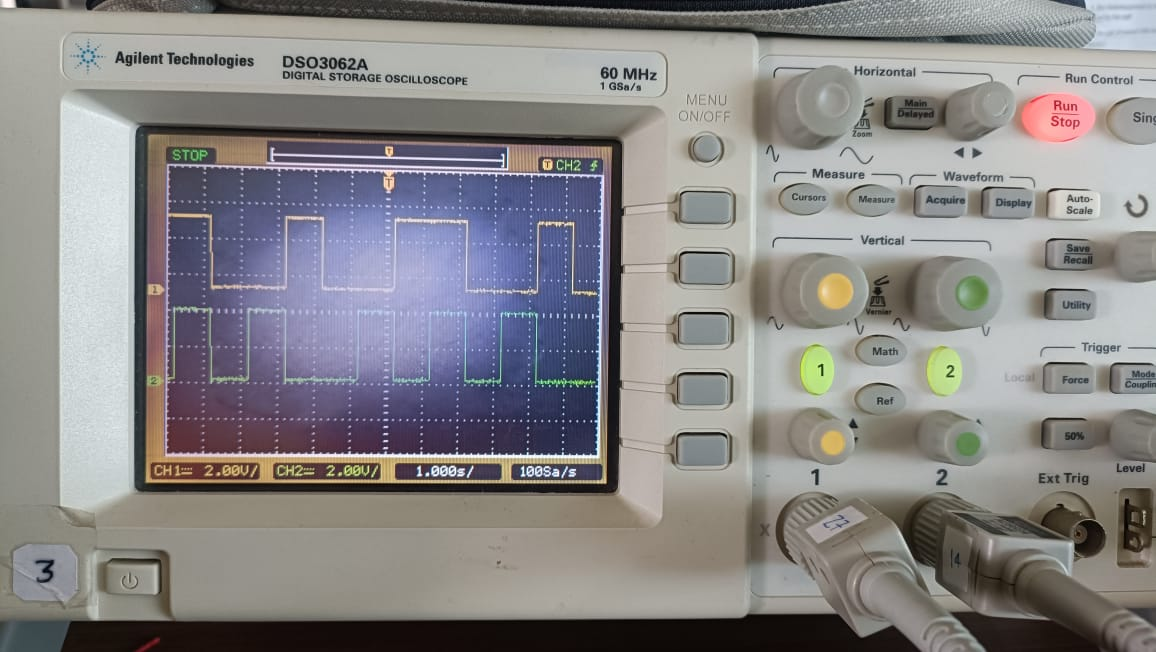
\includegraphics[width=0.7\textwidth]{figs/Q0Q1.jpeg} 
    \caption{Channel1-Q2,Channel2-Q1}
\end{figure}
\begin{figure}[H]
    \centering
    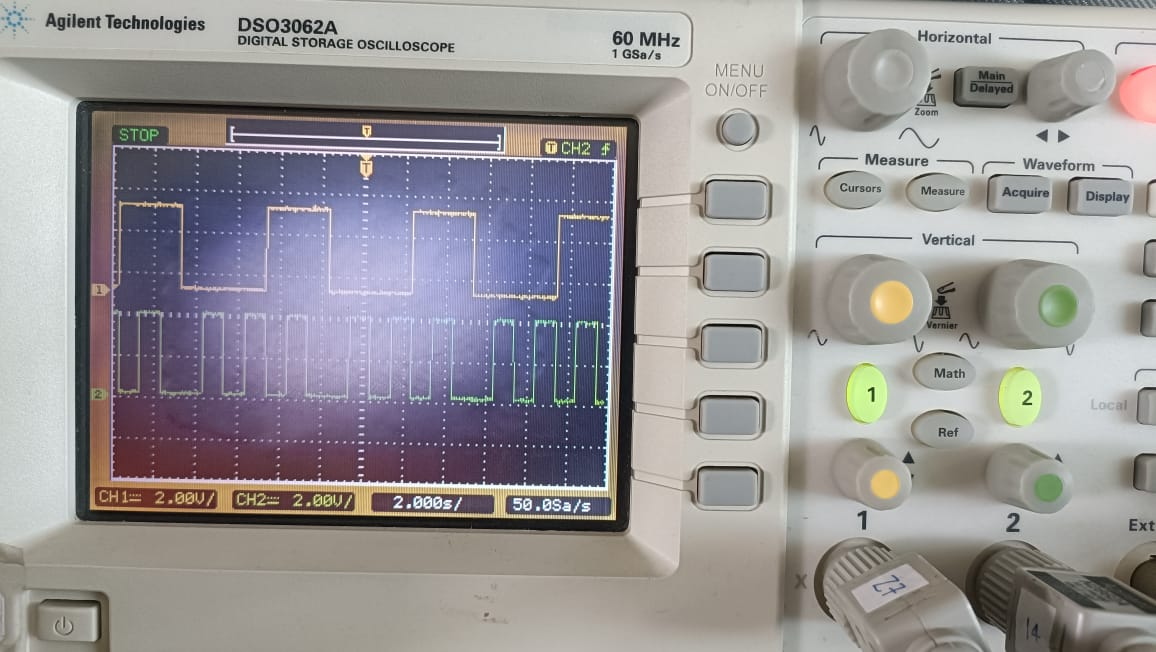
\includegraphics[width=0.7\textwidth]{figs/Q0Q2.jpeg} 
    \caption{Channel1-Q3,Channel2-Q1}
\end{figure}
\begin{figure}[H]
    \centering
    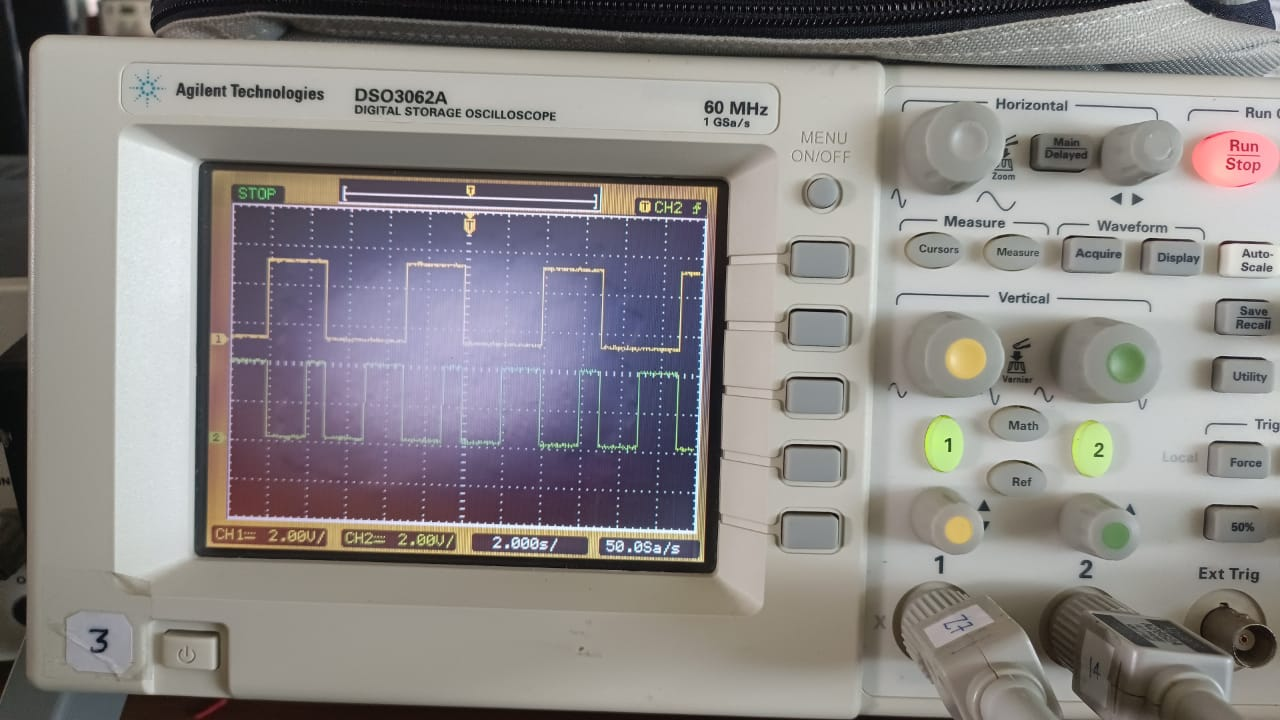
\includegraphics[width=0.7\textwidth]{figs/Q1Q2.jpeg} 
    \caption{Channel1-Q3,Channel2-Q2}
\end{figure}

\section{Arduino Clock Generation}
\begin{tcolorbox}[colback=boxbg,colframe=titlebg,title=Arduino Clock Generation Code,breakable]
\lstset{style=arduino}
\begin{lstlisting}
/*
 * MOD-7 Counter Clock Generator
 * This code generates a square wave clock signal for the MOD-7 counter
 * The frequency can be adjusted by changing the CLOCK_DELAY_MS constant
 */

const int CLOCK_PIN = 13;        // Clock output pin
const int CLOCK_DELAY_MS = 500;  // Half-period of clock in milliseconds
unsigned long clockCount = 0;    // Counter for clock pulses

void setup() {
  // Initialize serial communication for monitoring
  Serial.begin(9600);
  Serial.println("MOD-7 Counter Clock Generator");
  Serial.print("Clock Frequency: ");
  Serial.print(1000.0 / (2 * CLOCK_DELAY_MS));
  Serial.println(" Hz");
  
  // Configure clock pin as output
  pinMode(CLOCK_PIN, OUTPUT);
  digitalWrite(CLOCK_PIN, LOW);
}

void loop() {
  // Generate HIGH phase of clock
  digitalWrite(CLOCK_PIN, HIGH);
  Serial.print("Clock: HIGH | Count: ");
  Serial.println(clockCount);
  delay(CLOCK_DELAY_MS);
  
  // Generate LOW phase of clock
  digitalWrite(CLOCK_PIN, LOW);
  Serial.print("Clock: LOW  | Count: ");
  Serial.println(clockCount);
  delay(CLOCK_DELAY_MS);
  
  // Increment clock count for tracking
  clockCount++;
  
  // Reset counter visualization after reaching 6
  if (clockCount > 6) {
    clockCount = 0;
    Serial.println("-------- Counter Reset --------");
  }
}
\end{lstlisting}
\end{tcolorbox}

\section{Conclusion}
\begin{tcolorbox}[colback=boxbg,colframe=titlebg,title=Conclusion,breakable]
The MOD-7 asynchronous counter using T flip-flops (implemented with JK flip-flops) demonstrates several important concepts in digital electronics:

\begin{itemize}
    \item The practical implementation of T flip-flops using more common JK flip-flops
    \item The design and operation of asynchronous (ripple) counters
    \item The modification of a natural binary counter to a modulo-n counter using reset logic
    \item The ripple effect and associated timing considerations in asynchronous designs
\end{itemize}

The counter successfully counts from 0 to 6 before resetting to 0, driven by a clock signal generated by an Arduino. The oscilloscope measurements confirm the expected behavior, including the frequency division at each stage and the reset action.

While asynchronous counters are simple to design and implement, their timing limitations make them less suitable for high-speed applications. For higher frequencies, synchronous counter designs would be preferred to eliminate the ripple delay issues.
\end{tcolorbox}

\end{document}
